\documentclass{standalone}
\usepackage{tikz}
\usetikzlibrary{patterns, positioning}


\begin{document}
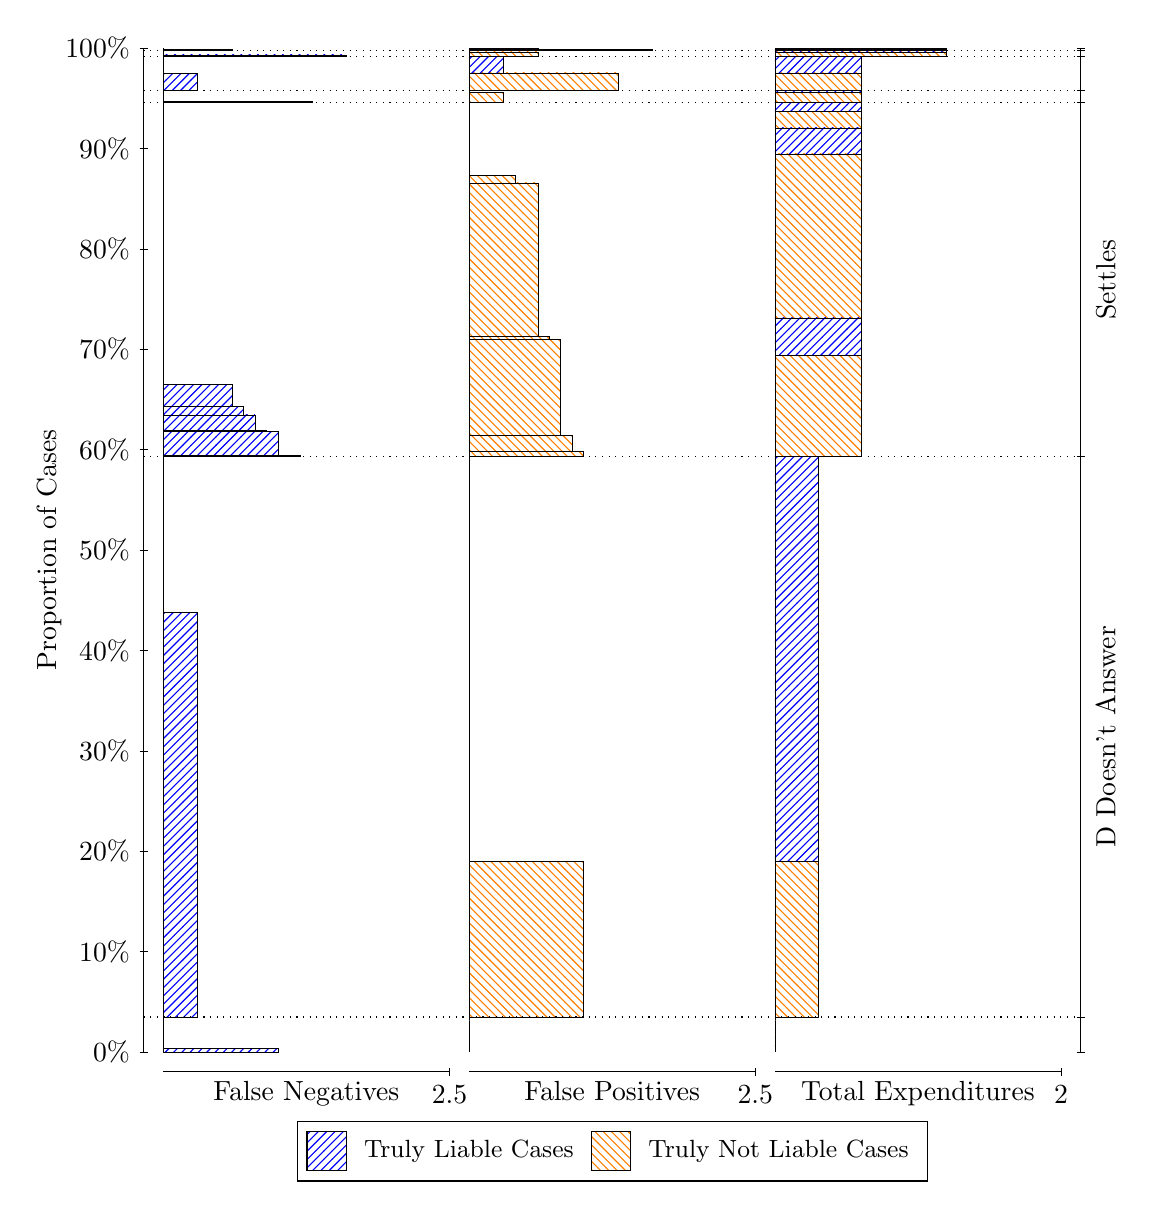
\begin{tikzpicture}
\draw[black, very thin] (1.5,1.75) -- (1.5,14.5);
\node[rotate=90, text=black, anchor=center] at (0.3, 8.125) {Proportion of Cases};
\draw[black, very thin] (1.45,1.75) -- (1.55,1.75);
\node[text=black, anchor=east] at (1.45, 1.75) {0\%};
\draw[black, very thin] (1.45,3.025) -- (1.55,3.025);
\node[text=black, anchor=east] at (1.45, 3.025) {10\%};
\draw[black, very thin] (1.45,4.3) -- (1.55,4.3);
\node[text=black, anchor=east] at (1.45, 4.3) {20\%};
\draw[black, very thin] (1.45,5.575) -- (1.55,5.575);
\node[text=black, anchor=east] at (1.45, 5.575) {30\%};
\draw[black, very thin] (1.45,6.85) -- (1.55,6.85);
\node[text=black, anchor=east] at (1.45, 6.85) {40\%};
\draw[black, very thin] (1.45,8.125) -- (1.55,8.125);
\node[text=black, anchor=east] at (1.45, 8.125) {50\%};
\draw[black, very thin] (1.45,9.4) -- (1.55,9.4);
\node[text=black, anchor=east] at (1.45, 9.4) {60\%};
\draw[black, very thin] (1.45,10.675) -- (1.55,10.675);
\node[text=black, anchor=east] at (1.45, 10.675) {70\%};
\draw[black, very thin] (1.45,11.95) -- (1.55,11.95);
\node[text=black, anchor=east] at (1.45, 11.95) {80\%};
\draw[black, very thin] (1.45,13.225) -- (1.55,13.225);
\node[text=black, anchor=east] at (1.45, 13.225) {90\%};
\draw[black, very thin] (1.45,14.5) -- (1.55,14.5);
\node[text=black, anchor=east] at (1.45, 14.5) {100\%};

\draw[black, very thin] (13.4,1.75) -- (13.4,14.5);
\draw[black, very thin] (13.35,1.75) -- (13.45,1.75);
\node[anchor=west] at (13.35, 1.75) {};
\draw[black, very thin] (13.35,2.1948) -- (13.45,2.1948);
\node[anchor=west] at (13.35, 2.1948) {};
\draw[black, very thin] (13.35,9.3098) -- (13.45,9.3098);
\node[anchor=west] at (13.35, 9.3098) {};
\draw[black, very thin] (13.35,13.805) -- (13.45,13.805);
\node[anchor=west] at (13.35, 13.805) {};
\draw[black, very thin] (13.35,13.96) -- (13.45,13.96);
\node[anchor=west] at (13.35, 13.96) {};
\draw[black, very thin] (13.35,14.397) -- (13.45,14.397);
\node[anchor=west] at (13.35, 14.397) {};
\draw[black, very thin] (13.35,14.468) -- (13.45,14.468);
\node[anchor=west] at (13.35, 14.468) {};
\draw[black, very thin] (13.35,14.5) -- (13.45,14.5);
\node[anchor=west] at (13.35, 14.5) {};

\draw[black, very thin, pattern color=blue, pattern=north east lines] (1.75,1.75) rectangle (3.2033,1.7968);
\draw[black, very thin, pattern color=orange, pattern=north west lines] (1.75,1.7968) rectangle (1.75,2.1948);
\draw[black, very thin, pattern color=blue, pattern=north east lines] (1.75,2.1948) rectangle (2.186,7.3365);
\draw[black, very thin, pattern color=orange, pattern=north west lines] (1.75,7.3365) rectangle (1.75,9.3098);
\draw[black, very thin, pattern color=blue, pattern=north east lines] (1.75,9.3098) rectangle (3.494,9.3255);
\draw[black, very thin, pattern color=blue, pattern=north east lines] (1.75,9.3255) rectangle (3.2033,9.6289);
\draw[black, very thin, pattern color=blue, pattern=north east lines] (1.75,9.6289) rectangle (3.058,9.6395);
\draw[black, very thin, pattern color=blue, pattern=north east lines] (1.75,9.6395) rectangle (2.9127,9.8402);
\draw[black, very thin, pattern color=blue, pattern=north east lines] (1.75,9.8402) rectangle (2.7673,9.952);
\draw[black, very thin, pattern color=blue, pattern=north east lines] (1.75,9.952) rectangle (2.622,10.229);
\draw[black, very thin, pattern color=orange, pattern=north west lines] (1.75,10.229) rectangle (1.75,13.805);
\draw[black, very thin, pattern color=blue, pattern=north east lines] (1.75,13.805) rectangle (3.6393,13.827);
\draw[black, very thin, pattern color=orange, pattern=north west lines] (1.75,13.827) rectangle (1.75,13.96);
\draw[black, very thin, pattern color=blue, pattern=north east lines] (1.75,13.96) rectangle (2.186,14.173);
\draw[black, very thin, pattern color=orange, pattern=north west lines] (1.75,14.173) rectangle (1.75,14.397);
\draw[black, very thin, pattern color=blue, pattern=north east lines] (1.75,14.397) rectangle (4.0753,14.413);
\draw[black, very thin, pattern color=orange, pattern=north west lines] (1.75,14.413) rectangle (1.75,14.468);
\draw[black, very thin, pattern color=blue, pattern=north east lines] (1.75,14.468) rectangle (2.622,14.484);
\draw[black, very thin, pattern color=orange, pattern=north west lines] (1.75,14.484) rectangle (1.75,14.5);
\draw[black, very thin, pattern color=orange, pattern=north west lines] (5.6333,1.75) rectangle (5.6333,2.148);
\draw[black, very thin, pattern color=blue, pattern=north east lines] (5.6333,2.148) rectangle (5.6333,2.1948);
\draw[black, very thin, pattern color=orange, pattern=north west lines] (5.6333,2.1948) rectangle (7.0867,4.1682);
\draw[black, very thin, pattern color=blue, pattern=north east lines] (5.6333,4.1682) rectangle (5.6333,9.3098);
\draw[black, very thin, pattern color=orange, pattern=north west lines] (5.6333,9.3098) rectangle (7.0867,9.3776);
\draw[black, very thin, pattern color=orange, pattern=north west lines] (5.6333,9.3776) rectangle (6.9413,9.5847);
\draw[black, very thin, pattern color=orange, pattern=north west lines] (5.6333,9.5847) rectangle (6.796,10.801);
\draw[black, very thin, pattern color=orange, pattern=north west lines] (5.6333,10.801) rectangle (6.6507,10.84);
\draw[black, very thin, pattern color=orange, pattern=north west lines] (5.6333,10.84) rectangle (6.5053,12.788);
\draw[black, very thin, pattern color=orange, pattern=north west lines] (5.6333,12.788) rectangle (6.2147,12.885);
\draw[black, very thin, pattern color=blue, pattern=north east lines] (5.6333,12.885) rectangle (5.6333,13.805);
\draw[black, very thin, pattern color=orange, pattern=north west lines] (5.6333,13.805) rectangle (6.0693,13.937);
\draw[black, very thin, pattern color=blue, pattern=north east lines] (5.6333,13.937) rectangle (5.6333,13.96);
\draw[black, very thin, pattern color=orange, pattern=north west lines] (5.6333,13.96) rectangle (7.5227,14.183);
\draw[black, very thin, pattern color=blue, pattern=north east lines] (5.6333,14.183) rectangle (6.0693,14.397);
\draw[black, very thin, pattern color=orange, pattern=north west lines] (5.6333,14.397) rectangle (6.5053,14.452);
\draw[black, very thin, pattern color=blue, pattern=north east lines] (5.6333,14.452) rectangle (5.6333,14.468);
\draw[black, very thin, pattern color=orange, pattern=north west lines] (5.6333,14.468) rectangle (7.9587,14.484);
\draw[black, very thin, pattern color=blue, pattern=north east lines] (5.6333,14.484) rectangle (6.5053,14.5);
\draw[black, very thin, pattern color=orange, pattern=north west lines] (9.5167,1.75) rectangle (9.5167,2.148);
\draw[black, very thin, pattern color=blue, pattern=north east lines] (9.5167,2.148) rectangle (9.5167,2.1948);
\draw[black, very thin, pattern color=orange, pattern=north west lines] (9.5167,2.1948) rectangle (10.062,4.1682);
\draw[black, very thin, pattern color=blue, pattern=north east lines] (9.5167,4.1682) rectangle (10.062,9.3098);
\draw[black, very thin, pattern color=orange, pattern=north west lines] (9.5167,9.3098) rectangle (10.607,10.594);
\draw[black, very thin, pattern color=blue, pattern=north east lines] (9.5167,10.594) rectangle (10.607,11.072);
\draw[black, very thin, pattern color=orange, pattern=north west lines] (9.5167,11.072) rectangle (10.607,13.156);
\draw[black, very thin, pattern color=blue, pattern=north east lines] (9.5167,13.156) rectangle (10.607,13.486);
\draw[black, very thin, pattern color=orange, pattern=north west lines] (9.5167,13.486) rectangle (10.607,13.693);
\draw[black, very thin, pattern color=blue, pattern=north east lines] (9.5167,13.693) rectangle (10.607,13.805);
\draw[black, very thin, pattern color=orange, pattern=north west lines] (9.5167,13.805) rectangle (10.607,13.937);
\draw[black, very thin, pattern color=blue, pattern=north east lines] (9.5167,13.937) rectangle (10.607,13.96);
\draw[black, very thin, pattern color=orange, pattern=north west lines] (9.5167,13.96) rectangle (10.607,14.183);
\draw[black, very thin, pattern color=blue, pattern=north east lines] (9.5167,14.183) rectangle (10.607,14.397);
\draw[black, very thin, pattern color=orange, pattern=north west lines] (9.5167,14.397) rectangle (11.697,14.452);
\draw[black, very thin, pattern color=blue, pattern=north east lines] (9.5167,14.452) rectangle (11.697,14.468);
\draw[black, very thin, pattern color=orange, pattern=north west lines] (9.5167,14.468) rectangle (11.697,14.484);
\draw[black, very thin, pattern color=blue, pattern=north east lines] (9.5167,14.484) rectangle (11.697,14.5);
\draw[black, dotted] (1.5,2.1948) -- (13.4,2.1948);
\draw[black, dotted] (1.5,9.3098) -- (13.4,9.3098);
\draw[black, dotted] (1.5,13.805) -- (13.4,13.805);
\draw[black, dotted] (1.5,13.96) -- (13.4,13.96);
\draw[black, dotted] (1.5,14.397) -- (13.4,14.397);
\draw[black, dotted] (1.5,14.468) -- (13.4,14.468);
\draw[black, very thin] (1.75,1.5) -- (5.3833,1.5);
\node[text=black, anchor=north] at (3.5667, 1.5) {False Negatives};
\draw[black, very thin] (5.3833,1.45) -- (5.3833,1.55);
\node[text=black, anchor=north] at (5.3833, 1.45) {2.5};

\draw[black, very thin] (5.6333,1.5) -- (9.2667,1.5);
\node[text=black, anchor=north] at (7.45, 1.5) {False Positives};
\draw[black, very thin] (9.2667,1.45) -- (9.2667,1.55);
\node[text=black, anchor=north] at (9.2667, 1.45) {2.5};

\draw[black, very thin] (9.5167,1.5) -- (13.15,1.5);
\node[text=black, anchor=north] at (11.333, 1.5) {Total Expenditures};
\draw[black, very thin] (13.15,1.45) -- (13.15,1.55);
\node[text=black, anchor=north] at (13.15, 1.45) {2};


\node[text=black, centered, rotate=90] at (13.72, 5.7523) {D Doesn't Answer};
\node[text=black, centered, rotate=90] at (13.72, 11.557) {Settles};





\draw (7.449999999999999,1.5) node[draw=none] (baseCoordinate) {};
\begin{scope}[align=center]
        \matrix[scale=0.5, draw=black, below=0.5cm of baseCoordinate, nodes={draw}, column sep=0.1cm]{
            \node[rectangle, draw, minimum width=0.5cm, minimum height=0.5cm, pattern color=blue, pattern=north east lines] {}; &
            \node[draw=none, font=\small, text=black] (B) {Truly Liable Cases}; &
            \node[rectangle, draw, minimum width=0.5cm, minimum height=0.5cm, pattern color=orange, pattern=north west lines] {}; &
            \node[draw=none, font=\small, text=black] (B) {Truly Not Liable Cases}; \\
            };
\end{scope}

\end{tikzpicture}
\end{document}